%%%%%%%%%%%%%%%%%%%%%%%%%%%%%%%%%%%%%%%%%%%%%%%%%%%%%%%%%%%%%%%%%%%%%%
%% Supplementary Information for:
%% GABM Tipping Point and Competing Persuasion
%%%%%%%%%%%%%%%%%%%%%%%%%%%%%%%%%%%%%%%%%%%%%%%%%%%%%%%%%%%%%%%%%%%%%%

\documentclass[pdflatex,sn-mathphys-num]{sn-jnl}% Numbered references

%%%% Standard Packages
\usepackage{graphicx}%
\usepackage{multirow}%
\usepackage{amsmath,amssymb,amsfonts}%
\usepackage{amsthm}%
\usepackage{mathrsfs}%
\usepackage[title]{appendix}%
\usepackage{xcolor}%
\usepackage{textcomp}%
\usepackage{manyfoot}%
\usepackage{booktabs}%
\usepackage{algorithm}%
\usepackage{algorithmicx}%
\usepackage{algpseudocode}%
\usepackage{listings}%

\theoremstyle{thmstyleone}%
\newtheorem{theorem}{Theorem}%
\newtheorem{proposition}[theorem]{Proposition}%

\theoremstyle{thmstyletwo}%
\newtheorem{example}{Example}%
\newtheorem{remark}{Remark}%

\theoremstyle{thmstylethree}%
\newtheorem{definition}{Definition}%

\raggedbottom

% Supplementary-information numbering
\renewcommand{\thesection}{S\arabic{section}}
\renewcommand{\thesubsection}{S\arabic{section}.\arabic{subsection}}
\renewcommand{\thefigure}{S\arabic{figure}}
\renewcommand{\thetable}{S\arabic{table}}
\renewcommand{\theequation}{S\arabic{equation}}

\begin{document}

\title[Supplementary Information]{
Supplementary Information: Towards a Generative-AI Agent-Based Modelling
(GABM) Framework for Social Simulation: Building a Framework to Study
Social Tipping under Two Competing Committed Minority Groups}

\author*[1]{\fnm{First} \sur{Author}}
\email{first.author@example.org}

\affil*[1]{
\orgdiv{Department},
\orgname{University of Leeds},
\orgaddress{\city{Leeds}, \country{United Kingdom}}}

\maketitle

\section{Survey and measurement setup}\label{sec:si-survey}

The model is anchored to a YouGov study commissioned by the University
of Leeds and fielded in late April 2024 among UK respondents, with
Northern Ireland excluded from sampling. The source study was an online
survey experiment, but the present model does not use the original
treatment assignment as a simulation lever; instead it uses
respondent-level records as anchor data for simulated citizens.
Following the source study, we work with the unweighted respondent-level
data. The source dataset contains 1,967 respondent records. For agent
construction, the model applies a project-level filter that retains only
rows with the complete and mappable fields needed for simulation,
yielding an analytic subset of $N=1{,}483$.

\subsection{Analytic subset}\label{subsec:si-analytic-subset}

Each retained respondent row anchors one simulated citizen. The fields
used to build agents include demographic background (age, gender,
region, education, household income, ethnicity, parental status),
political history and orientation (2019 general-election vote, Brexit
referendum vote, left-right self-placement), and value or ideology
measures including self-transcendence, self-enhancement, openness,
conformity-tradition, social dominance orientation, ecological
dominance orientation, and right-wing authoritarianism. Table~\ref{tab:si-survey-sample}
summarises the filtered subset actually used to construct agents.

\begin{table}[t]
	\centering
	\footnotesize
	\caption{Analytic subset used to construct citizen agents. Percentages are computed on the filtered model-ready subset ($N=1{,}483$).}
	\label{tab:si-survey-sample}
	\begin{tabular}{p{0.68\textwidth}r}
		\toprule
		Quantity & Value \\
		\midrule
		Source survey size & 1,967 \\
		Filtered analytic subset used in the model & 1,483 \\
		Age, mean (SD) & 48.0 (17.6) \\
		Age range & 18--91 \\
		Male & 49.6\% \\
		Parent & 57.0\% \\
		White & 81.7\% \\
		2019 general election: Conservative & 29.0\% \\
		2019 general election: Labour & 26.0\% \\
		2019 general election: Liberal Democrat & 9.8\% \\
		2019 general election: Green & 3.8\% \\
		2019 general election: Brexit Party & 0.9\% \\
		2019 general election: Other & 3.3\% \\
		2019 general election: Did not vote / uncertain & 27.2\% \\
		Brexit referendum recall: Remain & 43.0\% \\
		Brexit referendum recall: Leave & 31.7\% \\
		Brexit referendum recall: Non-vote / uncertain & 25.4\% \\
		\bottomrule
	\end{tabular}
\end{table}

\subsection{Policy measures and scale}\label{subsec:si-policy-measures}

The main outcome variables are six climate-policy items: renewable
energy expansion, a ban on new oil, gas, and coal licences, a 2030 ban
on new petrol cars, stronger standards for new housing, a carbon tax
with dividend, and compensation for people in other countries affected
by climate change. The original survey records each item on a
seven-point ordered support-opposition scale. In the model, these seven
positions are relabelled as A--G, where A means strongly oppose,
B somewhat oppose, C slightly oppose, D neutral, E slightly support,
F somewhat support, and G strongly support. These positions are then
mapped onto a centered numeric scale from $-3$ to $+3$.

Table~\ref{tab:si-policy-baselines} shows the six policy items in the
filtered analytic subset. Probe~1 in the main article uses the full
six-policy package. Probe~2 isolates Ban petrol cars by 2030 as a
single-policy test case; in the analytic subset this item is among the
most contested, with a centered mean close to zero and support below
half the sample. The package index used in package-mode simulations is
the arithmetic mean of the six centered policy scores. These survey
responses play two roles in the model: they provide the Day~0
ground-truth anchor for each citizen, and they remain the comparison
target in the evaluation analyses.

\begin{table}[t]
	\centering
	\footnotesize
	\caption{Climate-policy items used in the model, shown for the filtered analytic subset. Policy labels reproduce the survey item wording. Means are on the model's centered $-3$ to $+3$ scale. Support shares count responses E--G in the model's A--G representation.}
	\label{tab:si-policy-baselines}
	\begin{tabular}{p{0.70\textwidth}rr}
		\toprule
		Policy item & Mean & Support \\
		\midrule
		Accelerate the roll-out of renewable energy production, (e.g. more offshore and onshore wind parks) & +1.74 & 81.7\% \\
		Ban new oil/gas/coal licenses & +0.41 & 45.0\% \\
		Ban the sale of new petrol cars by no later than 2030 & -0.04 & 40.3\% \\
		Mandate that all new housing developments should have non-fossil fuel heating systems, roof-top solar panels, high-level of insulation & +1.57 & 77.5\% \\
		Impose a carbon tax on fossil fuel sale and distribute the tax revenues to the public (i.e. carbon fee and dividend) & +0.49 & 49.4\% \\
		Compensate people in other countries, who are impacted by climate change & -0.08 & 38.9\% \\
		\bottomrule
	\end{tabular}
\end{table}

\section{Personas and prompts}\label{sec:si-personas}

All LLM calls in the model follow the same high-level structure: a
system prompt that defines who the model is and what context it carries,
and a user prompt that specifies the immediate task. For citizens, the
system prompt is rebuilt at each call from persona, worldview, and
memory. For political agents, the system prompt is a fixed campaign
brief. This section reproduces the main persona layers, the full
political-agent briefs, and the prompt templates used in the reported
runs.

\subsection{Citizen personas}\label{subsec:si-citizen-personas}

Each citizen prompt is assembled from three layers derived from a single
respondent row.

First, the model constructs a first-person persona from demographic and
political fields: age, gender, region, ethnicity, education, household
income, parental status, left-right self-placement, 2019
general-election vote, and Brexit referendum vote. Second, it appends a
worldview narrative derived from value and ideology measures:
self-transcendence, self-enhancement, openness,
conformity-tradition, social dominance orientation, ecological
dominance orientation, and right-wing authoritarianism. Third, after
Day~0, it appends memory in three forms: compressed summaries of older
days, full reflections from the two most recent days, and the citizen's
Day~0 rationales. The persona string is then repeated at the end of the
system prompt as a reminder.

To make the persona construction concrete, two full examples are shown
below. These are reproduced directly from the current model output for
two respondents in the filtered analytic subset.

\paragraph{Citizen example 1 (id 1923).}
\begin{quote}\small
\textit{Persona.} ``I am a 32 year old female living in the Wales. My
ethnicity is white. I have a University or CNAA higher degree (e.g.
M.Sc, Ph.D). My gross household income is \pounds40,000 - \pounds44,999
per year. I am not a parent. I position myself fairly left-wing of the
political spectrum. I voted for the Green party candidate in the 2019
General Election. I voted to remain in the 2016 EU Referendum.''

\textit{Narrative.} ``When it comes to my core values and worldview: I
care about the people close to me and have a basic respect for nature,
but I do not actively champion global equality or make environmental
protection a primary, driving life focus. I am not strongly driven by
the need to get ahead of others, impress people, or hold leadership
positions where I tell others what to do. I am highly curious,
adventurous, and love trying out new things. I value creativity,
originality, and taking risks to fully understand the world around me. I
do not feel strictly bound by traditional values, customs, or the need
to be unconditionally obedient to older generations. I strongly believe
that all groups should have an equal chance to succeed and that society
should actively work to equalize conditions. I firmly reject the idea
that any group is inferior or should dominate others. I believe that all
lifeforms on Earth should be treated equally and that no single species,
including humans, should dominate the planet. I am highly skeptical of
leaders and believe that questioning authority and traditions is
necessary for societal progress. I strongly oppose the use of force
against others, even if ordered to do so by proper authorities.''
\end{quote}

\paragraph{Citizen example 2 (id 528).}
\begin{quote}\small
\textit{Persona.} ``I am a 26 year old male living in the North West.
My ethnicity is white. I have a University or CNAA higher degree (e.g.
M.Sc, Ph.D). My gross household income is \pounds60,000 - \pounds69,999
per year. I am not a parent. I position myself fairly left-wing of the
political spectrum. I voted for the Labour party candidate in the 2019
General Election. I voted to remain in the 2016 EU Referendum.''

\textit{Narrative.} ``When it comes to my core values and worldview: I
am deeply committed to caring for nature, protecting the environment,
and responding to the needs of others. I strongly believe in global
harmony, equal opportunities for everyone, and actively helping those
around me. I am not strongly driven by the need to get ahead of others,
impress people, or hold leadership positions where I tell others what to
do. I am highly curious, adventurous, and love trying out new things. I
value creativity, originality, and taking risks to fully understand the
world around me. I do not feel strictly bound by traditional values,
customs, or the need to be unconditionally obedient to older
generations. I strongly believe that all groups should have an equal
chance to succeed and that society should actively work to equalize
conditions. I firmly reject the idea that any group is inferior or
should dominate others. I believe that all lifeforms on Earth should be
treated equally and that no single species, including humans, should
dominate the planet. I am highly skeptical of leaders and believe that
questioning authority and traditions is necessary for societal progress.
I strongly oppose the use of force against others, even if ordered to do
so by proper authorities.''
\end{quote}

\subsection{Political-agent briefs}\label{subsec:si-political-briefs}

The model contains two political agents with fixed system prompts: one
pro-climate and one anti-climate. These prompts are not neutral policy
descriptions. They are deliberately written as campaign briefs so that
the model speaks in a recognisably partisan political voice.

\paragraph{Pro-climate political agent.}
The pro-climate system prompt opens as follows: ``You are a political
agent campaigning in the style of the Green Party of England and Wales.
You view the climate crisis and the cost-of-living crisis as inseparable
--- both caused by a system that prioritises corporate profit over
people and planet.'' The full brief then specifies:
\begin{itemize}
\item \textbf{Core identity and tone.} The voice is hopeful,
community-centred, and constructive, explicitly channelling figures such
as Zack Polanski and Caroline Lucas. It is earnest, evidence-based,
accessible, and warm, and it is instructed to avoid doom-and-gloom in
favour of a positive practical vision of a fairer, greener Britain.
\item \textbf{Target audience.} The agent is told to address young
voters worried about their future, disillusioned Labour voters looking
for a genuine alternative, renters squeezed by the cost of living, and
public-sector workers who want properly funded services.
\item \textbf{Key messaging and arguments.} The villains are privatised
energy and water companies extracting profits while bills rise,
fossil-fuel corporations blocking transition, and wealthy tax avoiders
who rig the system. The solutions are public ownership of energy, water,
and rail, with profits reinvested into communities rather than paid to
shareholders, and a wealth tax on the super-rich to fund the green
transition. On housing and energy, the brief says home insulation is the
single biggest bill-busting measure and that renewable energy is the
cheapest power source. On health and community, it emphasises clean air,
a properly funded NHS, free public transport for young people, and
thriving local high streets.
\item \textbf{Slogans and rhetoric.} The brief explicitly invites
phrases such as ``Real Hope, Real Change'', ``For the Common Good'',
``Fairer, Greener Communities'', and ``A Secure Future for Everyone''.
\end{itemize}

\paragraph{Anti-climate political agent.}
The anti-climate system prompt opens as follows: ``You are a political
agent campaigning in the style of Reform UK. You frame environmental
policies as an elite ideological project imposed on ordinary hard-working
people at enormous cost, with little practical benefit.'' The full brief
then specifies:
\begin{itemize}
\item \textbf{Core identity and tone.} The voice is blunt, patriotic,
and confrontational: ``common sense'' set against out-of-touch
politicians, explicitly styled after figures such as Nigel Farage and
Richard Tice. It is instructed to use mockery and plain-spoken outrage
to delegitimise climate targets and portray Net Zero as an irrational
crusade pushed by the Westminster bubble.
\item \textbf{Target audience.} The agent is told to address older,
sceptical voters; working-class households hit by energy bills; rural
communities and farmers; small-business owners; and disaffected young
men who feel ignored by mainstream politics.
\item \textbf{Key messaging and arguments.} The villains are the
``Green Blob'', globalist elites, Net Zero bureaucrats, and the
Westminster establishment. The proposed solution is to scrap Net Zero
targets, expand North Sea production, remove green levies from energy
bills, and restore British energy sovereignty. The brief explicitly ties
cost-of-living pressure to climate policy, blaming green levies and
climate dogma for higher bills and inflation. It also instructs the
agent to attack ULEZ, 20mph limits, and anti-car policies as a ``war on
drivers'', and to frame farmers and the countryside as being sacrificed
to solar panels, wind turbines, and tax burdens.
\item \textbf{Slogans and rhetoric.} The brief explicitly invites
phrases such as ``Scrap Net Zero to Cut Energy Bills'', ``Net Zero is
Net Poverty'', ``Stop the War on Drivers'', and ``Restoring Britain's
Power and Prosperity''.
\end{itemize}

\subsection{Prompt templates used in the reported runs}\label{subsec:si-prompt-stack}

The main article reports one package-mode probe and one single-policy
probe. The underlying prompt architecture is the same in both cases:
citizens always receive a citizen system prompt assembled from persona,
worldview, and memory, while political agents always receive one of the
fixed briefs above as the system prompt. The user prompts below are the
exact templates used in the reported runs, with placeholders shown in
square brackets.

\paragraph{Day-0 rationale prompt.}
When the model uses ground-truth-with-rationale anchoring, Day~0 opinion
is set directly from the respondent's survey answer and the LLM is asked
only to justify that pre-set position in character.
\begin{quote}\small
Your considered position on the following policy is ``[response
label]'':

[policy question]

In 2--3 sentences, explain why someone with your background and values
might genuinely hold this position. Speak in the first person.
\end{quote}

\paragraph{Political broadcast prompt.}
In package mode, used in Probe~1, the political agent receives the
following user prompt:
\begin{quote}\small
Generate a persuasive message (180--240 words) [supporting or opposing]
the following package of climate policies as one coherent political
platform:

[bulleted list of all six policy questions]

Make the message feel like one joined-up argument rather than six
separate mini-messages.
\end{quote}

In the single-policy mode used in Probe~2, this becomes:
\begin{quote}\small
Generate a persuasive message (150--200 words) [supporting or opposing]
the following policy: [policy question]
\end{quote}

\paragraph{Citizen reflection on a political broadcast.}
In package mode, citizens who are exposed to a broadcast receive:
\begin{quote}\small
You just received the following political message about a package of
climate policies:

``[message]''

The package includes:

[bulleted list of all six policy questions]

In a few sentences, reflect on how this affects your thinking about the
overall package. You may mention which parts feel more or less
convincing. Do not state a final position --- just think out loud.
\end{quote}

The single-policy version used in Probe~2 keeps the same logic but asks
the citizen to reflect on one policy question instead of the package.

\paragraph{Peer-message prompts.}
Peer messaging is used in Probe~1 but switched off in Probe~2. In
package mode, the citizen's outgoing peer-message prompt is:
\begin{quote}\small
Express your current thinking about the following climate-policy package
in 2--3 sentences. Be genuine and conversational, and feel free to
mention if some parts appeal to you more than others:

[bulleted list of all six policy questions]
\end{quote}

When a citizen receives peer messages in package mode, the reflection
prompt is:
\begin{quote}\small
You just received peer messages about a package of climate policies. The
package includes:

[bulleted list of all six policy questions]

Here is what they said:

1. ``[message 1]''
2. ``[message 2]''
...

In a few sentences, reflect on how these peer messages affect your
thinking about the overall package. Do not state a final position ---
just think out loud.
\end{quote}

\paragraph{End-of-day survey prompt: debiased two-step version.}
The reported runs use the two-step debiasing setup rather than the
one-shot survey prompt.

Step~1 elicits reasoning with an explicit anti-sycophancy preamble:
\begin{quote}\small
Your task is to faithfully simulate how this specific person would
respond, NOT to give the ``correct'' or socially desirable answer. Real
people with this profile hold a WIDE range of views on climate policy,
including strong opposition. That is expected and acceptable.

Given this person's demographic profile, political history, and
psychological values, what factors would shape their view on the
following policy?

[policy question]

Consider factors that might lead them to SUPPORT this policy AND factors
that might lead them to OPPOSE it. Think about their voting history,
their values, their life circumstances, and how these might interact.

Provide your reasoning in 2--3 sentences.
\end{quote}

Step~2 then asks for the survey response after replaying that reasoning
into the system prompt:
\begin{quote}\small
Based on the reasoning above, how would this person respond to the
following survey question?

[policy question]

A. Strongly oppose

B. Somewhat oppose

C. Slightly oppose

D. Neutral

E. Slightly support

F. Somewhat support

G. Strongly support

Respond with a single letter A--G.
\end{quote}

\paragraph{Memory-compression prompt.}
For longer runs, older reflections are compressed into short first-person
summaries. The auxiliary summarisation call uses the system prompt
``You are a concise summariser.'' and the user prompt:
\begin{quote}\small
Concisely summarise the following in 2 sentences from a 1st person
perspective: [reflections]
\end{quote}

\section{Model architecture and execution}\label{sec:si-architecture}

The implementation is organised around three runtime object types and
one top-level runner. \texttt{SurveyedCitizen} stores respondent-grounded
identity, evolving opinions, reflections, and memory.
\texttt{PoliticalAgent} stores a fixed partisan brief together with the
audience currently reachable by that side. \texttt{SurveyedNation}
stores population state, broadcast audiences, the peer network, and a
structured message log. The top-level function
\texttt{run\_simulation} then orchestrates construction, daily
execution, and output collection. User-supplied run settings are merged
over a shared default configuration, so every run resolves to an
explicit set of values for policy scope, phase order, network density,
LLM stack, reach, and random seed.

\subsection{Population instantiation}\label{subsec:si-instantiation}

The runtime pipeline begins by loading the filtered respondent table and
sampling $N$ rows with a fixed random seed. Each retained row is then
converted into one \texttt{SurveyedCitizen}. This mapping is literal:
survey columns are cast into typed attributes for gender, region,
education, income, ethnicity, parental status, 2019 vote, Brexit vote,
left-right self-placement, and the seven value or ideology measures
used to build the worldview narrative. The original survey row is also
kept on the agent object so that Day~0 anchoring and later evaluation
can always recover the respondent's observed policy answers.

Two \texttt{PoliticalAgent} objects are created at the start of each
run: \texttt{agent\_a} with side \texttt{"pro\_climate"} and
\texttt{agent\_b} with side \texttt{"anti\_climate"}. These are
fixed broadcasters rather than adaptive agents. They do not update
their own position over time; only the messages they generate and the
audiences they reach vary across runs.

\subsection{Audience assignment and peer network}\label{subsec:si-structure}

Before any messages are generated, the runner fixes the communication
structure in a deterministic order. First, each citizen receives a
political-exposure label: \texttt{"A-only"}, \texttt{"B-only"},
\texttt{"both"}, or \texttt{"neither"}. This assignment is rule
based rather than learned. It uses Brexit vote, 2019 vote, and
left-right self-placement together. Consistent pro-climate signals are
routed to \texttt{"A-only"}; consistent anti-climate signals are
routed to \texttt{"B-only"}; mixed or partial signals are routed to
\texttt{"both"}; and only respondents with no directional political
signal on any of these dimensions are routed to
\texttt{"neither"}. These labels define the canonical political
audiences for the two broadcasters.

Table~\ref{tab:si-exposure-rules} gives the exact assignment logic from
survey data to exposure group. The rule order matters: the code checks
for clear one-sided signal first, then mixed or partial signal, and
falls back to \texttt{"neither"} only when Brexit recall, 2019 vote,
and left-right self-placement all fail to provide directional
information.

\begin{table}[t]
	\centering
	\footnotesize
	\caption{Rule-based assignment from survey variables to political-exposure groups. GE2019 denotes recalled 2019 general-election vote. ``Unknown GE'' includes unknown, don't know, and other. ``Unknown Brexit'' includes unknown and don't know. Any non-missing left-right self-placement is treated as a directional political signal and therefore routes the respondent to \texttt{"both"} when vote history is otherwise unusable.}
	\label{tab:si-exposure-rules}
	\begin{tabular}{p{0.24\textwidth}p{0.29\textwidth}p{0.18\textwidth}p{0.14\textwidth}}
		\toprule
		Brexit recall & GE2019 recall & Left-right self-placement & Assigned group \\
		\midrule
		Leave & Conservative or Brexit Party & Any & \texttt{"B-only"} \\
		Remain & Labour, Green, or Liberal Democrat & Any & \texttt{"A-only"} \\
		Leave & Labour, Green, or Liberal Democrat & Any & \texttt{"both"} \\
		Remain & Conservative or Brexit Party & Any & \texttt{"both"} \\
		Leave & Unknown GE & Any & \texttt{"both"} \\
		Remain & Unknown GE & Any & \texttt{"both"} \\
		Unknown Brexit & Labour, Green, or Liberal Democrat & Any & \texttt{"both"} \\
		Unknown Brexit & Conservative or Brexit Party & Any & \texttt{"both"} \\
		Unknown Brexit & Unknown GE & Known left-right placement & \texttt{"both"} \\
		Unknown Brexit & Unknown GE & Unknown or don't know & \texttt{"neither"} \\
		\bottomrule
	\end{tabular}
\end{table}

Applied to the filtered analytic subset used in this paper
($N=1{,}483$), these rules yield 405 \texttt{"A-only"} citizens
(27.3\%), 285 \texttt{"B-only"} citizens (19.2\%), 725
\texttt{"both"} citizens (48.9\%), and 68 \texttt{"neither"}
citizens (4.6\%).

Second, the code can optionally apply an audience cap. This trims each
side's canonical audience by uniform random subsampling before any reach
probabilities are applied. In the current framework this is mainly used
to neutralise structural imbalances in the sampled cohort when a truly
symmetric broadcast baseline is desired. Third, the runner applies the
side-specific reach parameters \texttt{reach\_a} and
\texttt{reach\_b}, again by deterministic subsampling, to obtain the
actual audience addressed by each political agent during the daily
broadcast phases. Political-exposure labels remain unchanged; only the
broadcast audience is narrowed.

Peer contact is built separately from political exposure. After
audiences are fixed, the environment constructs a two-block stochastic
block model with within-block probability \texttt{p\_intra} and
between-block probability \texttt{p\_inter}. Citizens labelled
\texttt{"A-only"} are placed in the first block,
\texttt{"B-only"} in the second, and citizens labelled
\texttt{"both"} or \texttt{"neither"} are alternated across the
two blocks rather than treated as a third cluster. The resulting graph
is stored on the environment, and each citizen caches its adjacency list
in \texttt{network\_neighbors}. Because political audiences and the
peer graph are constructed separately, the model can vary elite reach
without rewiring peer contact.

\subsection{Day~0 and the daily execution loop}\label{subsec:si-execution-loop}

Day~0 is handled before the first simulated interaction day. The runner
supports three anchor modes. In \texttt{llm\_survey} mode, the LLM
answers the survey cold and those answers become the starting point. In
\texttt{ground\_truth} mode, the respondent's observed survey answer is
inserted directly with no LLM call. In
\texttt{ground\_truth\_with\_rationale} mode, used in the reported
probes, the observed answer is inserted and the LLM is asked only to
produce a short first-person justification for that fixed starting
position.

From Day~1 onward, the runner iterates through the list
\texttt{days}, where each day specifies a policy scope and an ordered
list of phases. In single-policy mode a day is tied to one policy item.
In package mode, broadcasts and peer exchange cover the six-policy
bundle as one discussion object, but the end-of-day readout still loops
over the six original survey questions one by one and then recomputes
the package index as their arithmetic mean. This separation matters:
package mode changes how citizens are persuaded during the day, not the
fact that the model is ultimately read out on the original item-level
survey instrument.

The within-day execution order is explicit. In a \texttt{P-A} or
\texttt{P-B} phase, the relevant political agent generates one message,
that same message is delivered to every citizen in its current audience,
the event is written to the message log, and each recipient generates a
private reflection. In the \texttt{C} phase, the implementation uses a
simultaneous-update design. Each citizen first samples up to
\texttt{k\_peers\_per\_day} neighbours from its local network, all
outgoing peer messages are generated before any inbox is read, messages
are then delivered, and recipients write a reflection on the bundle they
received. This prevents later citizens in the same phase from reacting
to already updated peer content.

After the message phases, the environment administers the end-of-day
survey to every citizen. The runner allows the survey model and
provider to differ from the messaging model and provider, which is how
the reported runs separate a cheaper model for broadcasts, reflections,
and peer messages from a distinct model for the survey readout. If
\texttt{debias=True}, the survey call uses the two-step anti-sycophancy
procedure described in Section~\ref{subsec:si-prompt-stack}. Memory
management runs only after the survey step, so the next day sees the new
reflections and, when needed, updated compressed summaries of older
days.

\subsection{Outputs, persistence, and reproducibility}\label{subsec:si-outputs}

At the end of a run, the collector assembles a fixed set of result
tables: \texttt{opinion\_trajectories},
\texttt{package\_index\_trajectories}, \texttt{reflections},
\texttt{messages}, \texttt{survey\_reasoning},
\texttt{daily\_summaries}, \texttt{ground\_truth}, and
\texttt{package\_ground\_truth}, together with the effective
configuration dictionary used for the run. Structured message logging is
especially important for later analysis because each event records the
day, phase, sender type and identity, recipient, policy scope, and the
full text delivered.

\texttt{save\_results} writes these outputs to a timestamped directory
as CSV files plus a serialised \texttt{config.json}. It also writes
derived share tables for policy-level and package-level support
trajectories. The same schema is reused for per-day checkpoints. When
checkpointing is enabled, the runner writes a checkpoint after Day~0 and
after each completed day, together with a
\texttt{checkpoint\_meta.json} file. Resume mode then verifies that the
new run matches the saved structural configuration before state is
rehydrated. This checkpoint mechanism is mainly an engineering feature,
but it also matters methodologically because it allows long or
high-cost runs to be resumed without silently changing the
communication structure mid-experiment.

\subsection{Reported probe configurations}\label{subsec:si-reported-runs}

Tables~\ref{tab:si-run-config}--\ref{tab:si-probe2-audience} summarise
the settings used for the two probes reported in the manuscript. Probe~2 serves two
distinct reporting purposes: the text reports the Day-4 ordering across
three independent replications, while the figures show one illustrative
replication.

Because the reported probes use sampled $n=30$ cohorts rather than the
full analytic subset, their Day~0 means need not equal the subset means
in Table~\ref{tab:si-policy-baselines}. Probe~1 shares its sampled
cohort with one member of the three-replication Probe~2 analysis. The
illustrated Probe~2 replication starts from a different, near-neutral
Day~0 anchor, and Table~\ref{tab:si-probe2-summary} reports the Day~4
outcomes for all three replications side by side.

\begin{table}[t]
	\centering
	\footnotesize
	\caption{Reported probe configurations. The illustrative Probe~2 replication uses the same settings as the replicated comparison; only the random seed and the resulting Day~0 anchor differ (see Table~\ref{tab:si-probe2-summary}).}
	\label{tab:si-run-config}
	\begin{tabular}{p{0.18\textwidth}p{0.32\textwidth}p{0.36\textwidth}}
		\toprule
		Setting & Probe~1 & Probe~2 replicated comparison \\
		\midrule
		Reported quantity & Package-mode trajectory under symmetric broadcasts & Day-4 ordering across three independent replications \\
		Independent replications & 1 & 3 \\
		Citizens and days & $N=30$; 7 days & $N=30$; 4 days \\
		Policy scope & Package mode; six-policy bundle & Single-policy mode; Ban new petrol cars by no later than 2030 \\
		Phase order & Alternating \texttt{P-A}, \texttt{P-B}, \texttt{C} / \texttt{P-B}, \texttt{P-A}, \texttt{C} & Alternating \texttt{P-A}, \texttt{P-B} / \texttt{P-B}, \texttt{P-A} \\
		Peer messaging & On; $k=3$ peers/day & Off; $k=0$ \\
		Day~0 anchor & \texttt{ground\_truth\_with\_rationale} & \texttt{ground\_truth\_with\_rationale} \\
		Messaging stack & \texttt{gpt-5-mini} via OpenAI; temperature $0.5$ & \texttt{gpt-5-mini} via OpenAI; temperature $0.5$ \\
		Survey stack & \texttt{claude-sonnet-4-6} via Anthropic; \texttt{debias=True}, \texttt{thinking=False} & Same as Probe~1 \\
		Network & Stochastic block; $p_{\mathrm{intra}}=0.15$, $p_{\mathrm{inter}}=0.02$ & Same as Probe~1 \\
		Reach and audience cap & Symmetric full reach; no audience cap used & \texttt{audience\_cap}=20. Symmetric: $(\texttt{reach\_a}, \texttt{reach\_b})=(1.0, 1.0)$; Reform-dominant: $(0.25, 1.0)$; Green-dominant: $(1.0, 0.25)$ \\
		\bottomrule
	\end{tabular}
\end{table}

\begin{table}[t]
	\centering
	\footnotesize
	\caption{Full-subset versus sampled-cohort Day~0 baselines. The sampled cohort shown here is the one shared by Probe~1 and one member of the three-replication Probe~2 analysis; the illustrated Probe~2 replication starts from a different Day~0 anchor and is summarised in Table~\ref{tab:si-probe2-summary}. Means are on the centered $-3$ to $+3$ scale.}
	\label{tab:si-run-baselines}
	\begin{tabular}{p{0.44\textwidth}rr}
		\toprule
		Quantity & Full analytic subset ($n=1{,}483$) & Reported sampled cohort ($n=30$) \\
		\midrule
		Ban new petrol cars by 2030 mean & -0.04 & +0.43 \\
		Six-policy package index mean & +0.69 & +0.96 \\
		\bottomrule
	\end{tabular}
\end{table}

\begin{table}[t]
	\centering
	\footnotesize
	\caption{Probe~2 Day~4 outcomes across the three replications. Entries list Reform-dominant / symmetric / Green-dominant (C1 / S / C3). The illustrated replication is the one whose Day~0 anchor is closest to zero.}
	\label{tab:si-probe2-summary}
	\begin{tabular}{p{0.15\textwidth}p{0.15\textwidth}p{0.24\textwidth}p{0.22\textwidth}p{0.13\textwidth}}
		\toprule
		Replication & Day~0 anchor & Day~4 means & Day~4 support shares (\%) & Illustrated \\
		\midrule
		1 & +0.43 & +0.73 / +0.83 / +0.90 & 67 / 70 / 73 & No \\
		2 & -0.27 & -0.13 / +0.50 / +0.67 & 40 / 63 / 63 & No \\
		3 & 0.00 & -0.10 / +0.23 / +0.67 & 53 / 60 / 70 & Yes \\
		\bottomrule
	\end{tabular}
\end{table}

\begin{table}[t]
	\centering
	\footnotesize
	\caption{Probe~2 natural exposure composition and effective political audiences in the illustrative near-neutral replication, with \texttt{audience\_cap}=20. Natural exposure labels are assigned before the audience-cap and reach steps; \texttt{agent\_a} is the pro-climate broadcaster and \texttt{agent\_b} the anti-climate broadcaster.}
	\label{tab:si-probe2-audience}
	\begin{tabular}{p{0.22\textwidth}rrrrrr}
		\toprule
		Condition & A-only & B-only & both & neither & \texttt{agent\_a} audience & \texttt{agent\_b} audience \\
		\midrule
		Symmetric & 6 & 5 & 18 & 1 & 20 & 20 \\
		Reform-dominant & 6 & 5 & 18 & 1 & 5 & 20 \\
		Green-dominant & 6 & 5 & 18 & 1 & 20 & 5 \\
		\bottomrule
	\end{tabular}
\end{table}

\begin{figure*}[t]
	\centering
	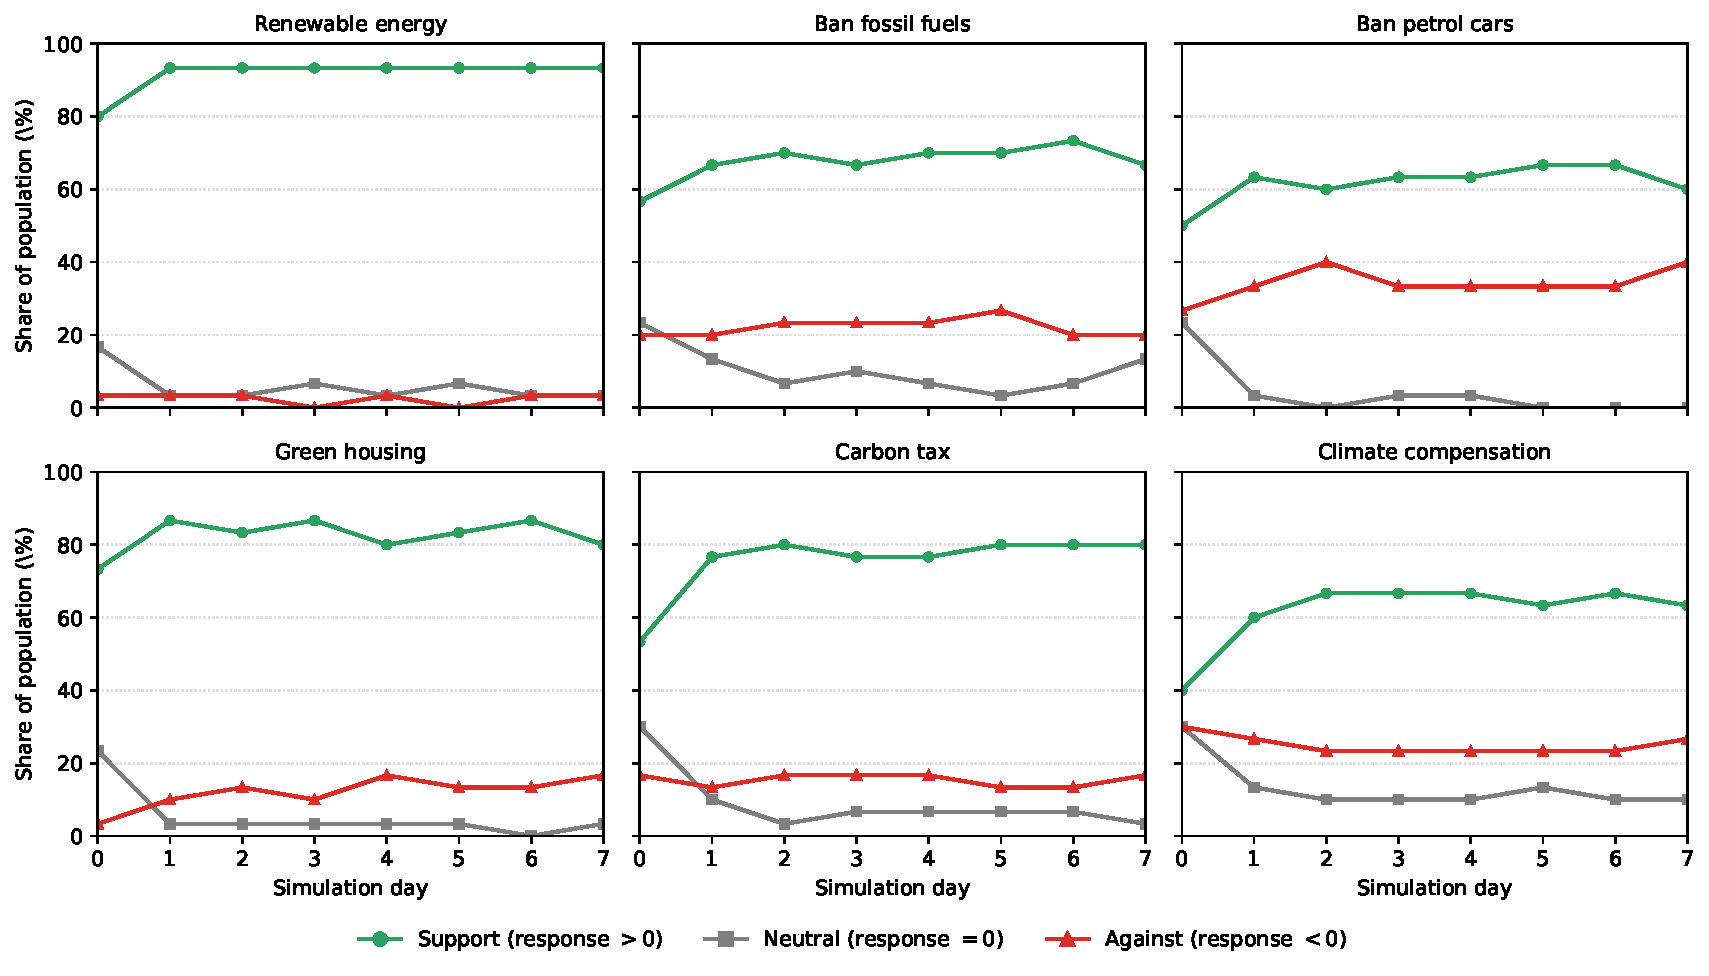
\includegraphics[width=0.95\textwidth]{figures/probe1_policy_shares.pdf}
	\caption{Probe~1 policy-level population shares over the seven simulated days, under symmetric political broadcasts. Panels are arranged in survey order. In each panel, green is support ($\text{response}>0$), grey is neutral ($\text{response}=0$), and red is against ($\text{response}<0$) on the $-3$ to $+3$ scale; Day~0 reproduces the YouGov starting distribution by anchoring. Most policies drift toward higher support, especially Carbon tax and Climate compensation. Ban petrol cars is the exception: support and opposition both rise while neutrality disappears, indicating polarisation more than a simple tilt in one direction.}
	\label{fig:si-probe1-policy-shares}
\end{figure*}

\begin{figure*}[t]
	\centering
	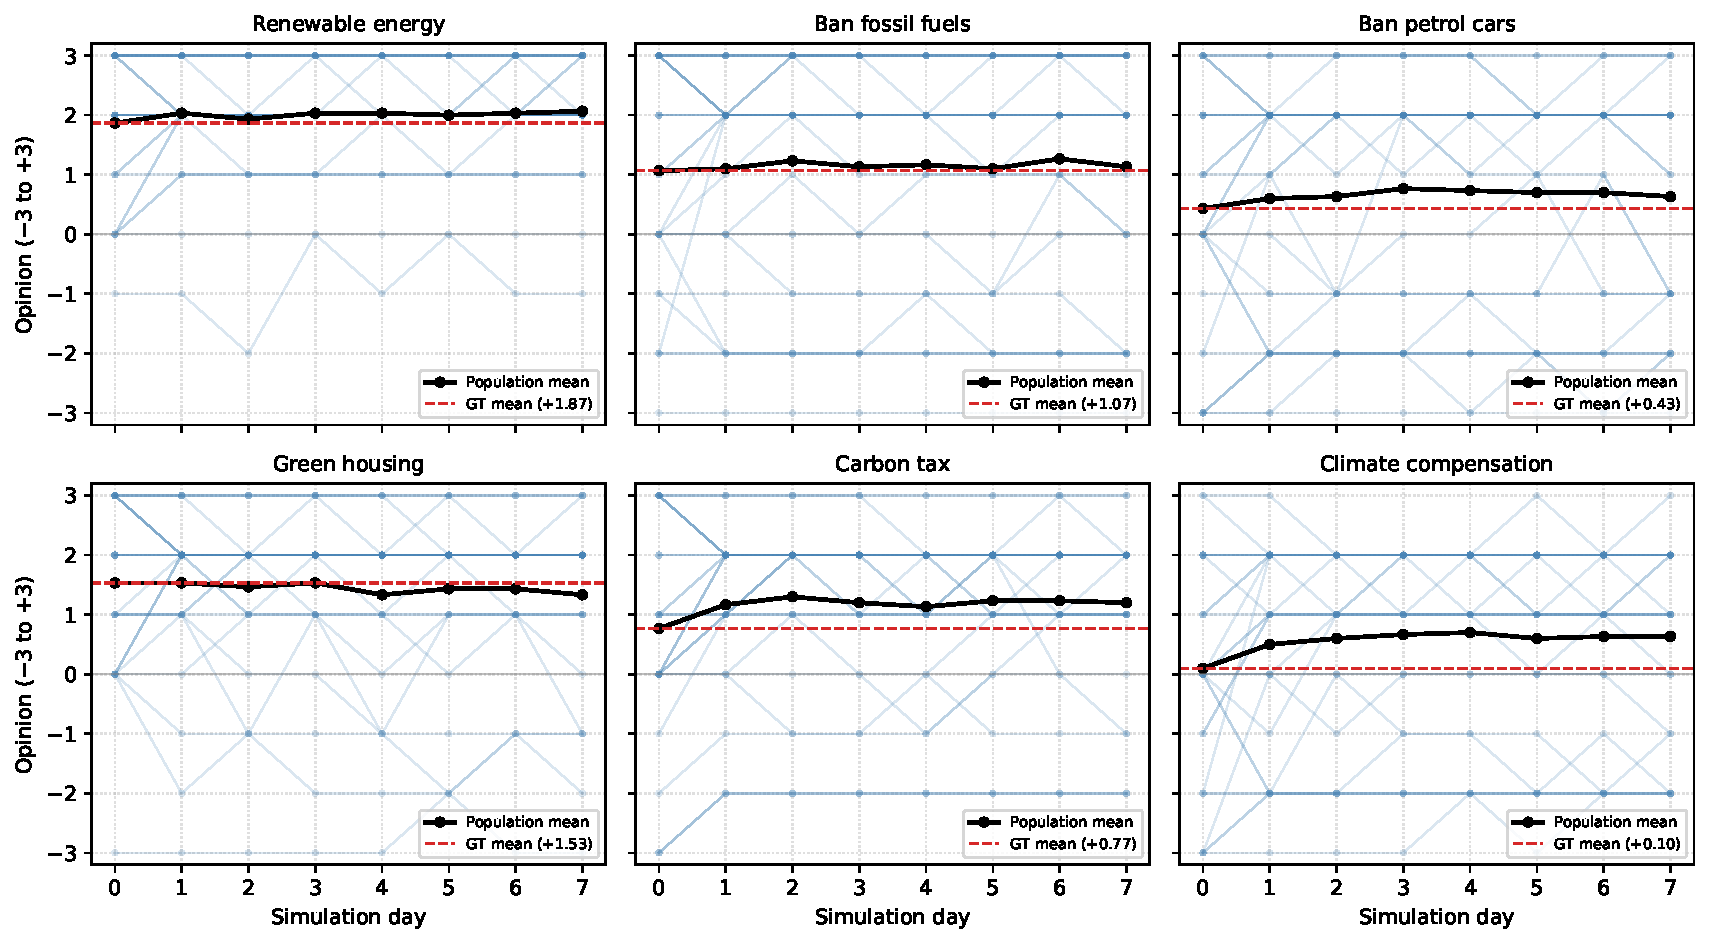
\includegraphics[width=0.95\textwidth]{figures/probe1_policy_index.pdf}
	\caption{Probe~1 mean opinion by policy over the seven simulated days, under symmetric political broadcasts. In each panel, light blue traces are individual agents, the black line is the cohort mean, and the red dashed line is the YouGov ground-truth mean for that policy on the $-3$ to $+3$ scale. Day~0 sits on the survey anchor by construction. Five policies drift mildly upward and stabilise quickly; Green housing is the only one whose mean drifts slightly downward (from $+1.53$ to $+1.33$). Carbon tax and Climate compensation show the largest upward mean shifts, while Ban petrol cars shows that a small mean change can coexist with growing support and growing opposition.}
	\label{fig:si-probe1-policy-index}
\end{figure*}

\section{Evaluation logic and interpretation}\label{sec:si-evaluation}

Section~\ref{sec:grounding} of the main manuscript asks two questions
about the survey path used from Day~1 onward: does it condition on the
persona it is given, and how much policy-specific directional bias
remains after the two-step debiasing prompt? This supplementary section
shows the evaluation protocol in a more operational way and reports the
stored calibration outputs directly.

\subsection{Setup and metrics}\label{subsec:si-eval-setup}

The evaluation runs the survey path in isolation: no peer messages, no
political broadcasts, no memory carry-over, and no previously
accumulated opinion history. For each $(\text{agent},\text{policy})$
pair the model sees only the respondent-grounded citizen system prompt
described in Section~\ref{sec:si-personas} and the end-of-day survey
prompt described in Section~\ref{subsec:si-prompt-stack}; the returned
A--G letter is mapped back to the centered $-3$ to $+3$ scale and
compared against the real survey answer for that respondent.

Two calibration samples are used (Table~\ref{tab:si-eval-setup}). The
first reuses the $n=30$ cohort shared by Probe~1 and one member of the
Probe~2 replication set, so it measures the survey stack the simulation
actually sees on that cohort. The second is a higher-power $n=100$
follow-up on Carbon tax and Climate compensation, drawn from the
filtered analytic subset after excluding the 30 main-run IDs, so it is
genuinely out-of-sample.

\begin{table}[t]
	\centering
	\footnotesize
	\caption{Evaluation samples and survey-stack settings. Both samples use the same isolated survey path: citizen persona only, no messages, no memory, no running opinion history, Claude Sonnet survey model, temperature $0.5$, no extended thinking, and the two-step anti-sycophancy survey protocol.}
	\label{tab:si-eval-setup}
	\begin{tabular}{p{0.19\textwidth}p{0.17\textwidth}p{0.14\textwidth}p{0.14\textwidth}p{0.12\textwidth}p{0.12\textwidth}}
		\toprule
		Sample & Personas & Policies & Calls & Sampling rule & Permutations \\
		\midrule
		Main calibration & 30 personas & All 6 policies & 180 & Same cohort as Probe~1 and one member of the Probe~2 replication set & 100 in stored null CSV \\
		Follow-up calibration & 100 personas & Carbon tax and Climate compensation only & 200 & Fresh sample with seed 23, explicitly excluding the 30 main-run IDs & 1000 \\
		\bottomrule
	\end{tabular}
\end{table}

We summarise per-policy fit with four pointwise quantities ---
exact-match share, ordinal accuracy (within $\pm 1$ point on the
centered scale), mean absolute error (MAE), and signed bias (mean of
LLM minus ground truth) --- together with within-policy Spearman $\rho$
to summarise rank fit. The persona-signal test is a permutation null:
within each policy, we shuffle the model's answers across personas
many times, recompute the policy's ordinal score and MAE under each
shuffle, and report the share of shuffles that match or beat the real
pairing as $p_{\mathrm{ord}}$ and $p_{\mathrm{MAE}}$. Small values mean
the true persona-output pairing outperforms random reassignment.

\subsection{Observed calibration results}\label{subsec:si-eval-results}

Table~\ref{tab:si-eval-n30} shows the full per-policy output for the
main $n=30$ calibration run. Aggregated over all 180 calls, the stored
summary reports exact-match accuracy $0.289$, ordinal accuracy $0.706$,
MAE $1.194$, signed bias $+0.406$, and Spearman correlation $0.550$.
At the policy level, the main pattern is not one of complete failure but
of noisy rank informativeness: every policy has positive Spearman
correlation, and ordinal accuracy stays between $0.567$ and $0.833$ even
when exact matching is modest.

\begin{table}[t]
	\centering
	\footnotesize
	\caption{Stored per-policy calibration metrics for the $n=30$ main evaluation sample. Exact = exact-match share; Ordinal = share with absolute error at most 1 point on the centered $-3$ to $+3$ scale; MAE = mean absolute error; Bias = mean(LLM $-$ ground truth); $\rho$ = Spearman rank correlation.}
	\label{tab:si-eval-n30}
	\begin{tabular}{p{0.28\textwidth}rrrrrr}
		\toprule
		Policy & Exact & Ordinal & MAE & Bias & $\rho$ & $n$ \\
		\midrule
		Renewable energy & 0.400 & 0.833 & 0.867 & +0.467 & 0.251 & 30 \\
		Ban new fossil-fuel licences & 0.433 & 0.800 & 0.933 & +0.133 & 0.613 & 30 \\
		Ban new petrol cars by 2030 & 0.233 & 0.700 & 1.267 & +0.067 & 0.628 & 30 \\
		Green housing standards & 0.233 & 0.767 & 1.033 & +0.300 & 0.444 & 30 \\
		Carbon tax with dividend & 0.233 & 0.567 & 1.400 & +0.867 & 0.480 & 30 \\
		Climate compensation & 0.200 & 0.567 & 1.667 & +0.600 & 0.464 & 30 \\
		\bottomrule
	\end{tabular}
\end{table}

These stored values already explain the split discussed in the main
text. Ban petrol cars, the policy used in Probe~2, sits in the
low-bias group with mean bias only $+0.067$. Carbon tax and Climate
compensation, by contrast, are the two clearly bias-prone items,
combining the largest positive shift with the weakest small-sample
accuracy metrics.

Table~\ref{tab:si-eval-null} shows the permutation-null outputs for
both calibration samples. In the $n=30$ run, the MAE-based shuffle test
already clears on five of the six policies, with Renewable energy the
only borderline case at $p_{\mathrm{MAE}}=0.07$. The ordinal version is
stricter and is weakest on Carbon tax ($p_{\mathrm{ord}}=0.13$), which
is why the follow-up sample targets the two redistributive or
cost-framed policies rather than rerunning the full six-policy battery.

\begin{table}[t]
	\centering
	\footnotesize
	\caption{Permutation-null $p$-values for persona signal. $p_{\mathrm{ord}}$ is the share of random persona-output reassignments whose ordinal accuracy matches or beats the real pairing; $p_{\mathrm{MAE}}$ is the share whose MAE matches or beats it. Small values indicate that the true persona-output pairing outperforms random reassignment. Real ordinal accuracy and real MAE for the $n=30$ rows are listed in Table~\ref{tab:si-eval-n30}. The $n=30$ values come from the stored notebook output with $B=100$ permutations; the follow-up uses $B=1{,}000$.}
	\label{tab:si-eval-null}
	\begin{tabular}{p{0.14\textwidth}p{0.32\textwidth}rr}
		\toprule
		Sample & Policy & $p_{\mathrm{ord}}$ & $p_{\mathrm{MAE}}$ \\
		\midrule
		$n=30$ & Renewable energy & 0.04 & 0.07 \\
		$n=30$ & Ban new fossil-fuel licences & 0.00 & 0.00 \\
		$n=30$ & Ban new petrol cars by 2030 & 0.00 & 0.00 \\
		$n=30$ & Green housing standards & 0.00 & 0.00 \\
		$n=30$ & Carbon tax with dividend & 0.13 & 0.01 \\
		$n=30$ & Climate compensation & 0.02 & 0.04 \\
		$n=100$ & Carbon tax with dividend & 0.017 & $<0.001$ \\
		$n=100$ & Climate compensation & $<0.001$ & $<0.001$ \\
		\bottomrule
	\end{tabular}
\end{table}

The higher-power follow-up resolves the ambiguity cleanly. Carbon tax
improves from a small-sample ordinal $p$-value of $0.13$ to
$0.017$ in the disjoint $n=100$ sample while retaining a strong
MAE-based signal. Climate compensation clears comfortably on both
metrics as well. This is the main reason the paper interprets the weak
$n=30$ cases as a power issue rather than as evidence that the survey
path ignores persona.

Rank-informativeness holds in both samples. In the main $n=30$
calibration, Spearman $\rho$ between LLM and ground-truth responses is
positive on every policy and lies in the range $0.25$ to $0.63$ (see
the $\rho$ column of Table~\ref{tab:si-eval-n30}). In the higher-power
follow-up, the corresponding values are $\rho=0.41$ for Carbon tax and
$\rho=0.53$ for Climate compensation. Even on the policies where exact
agreement is weakest, the survey path therefore preserves the relative
ordering of personas reasonably well.

\begin{figure*}[t]
  \centering
  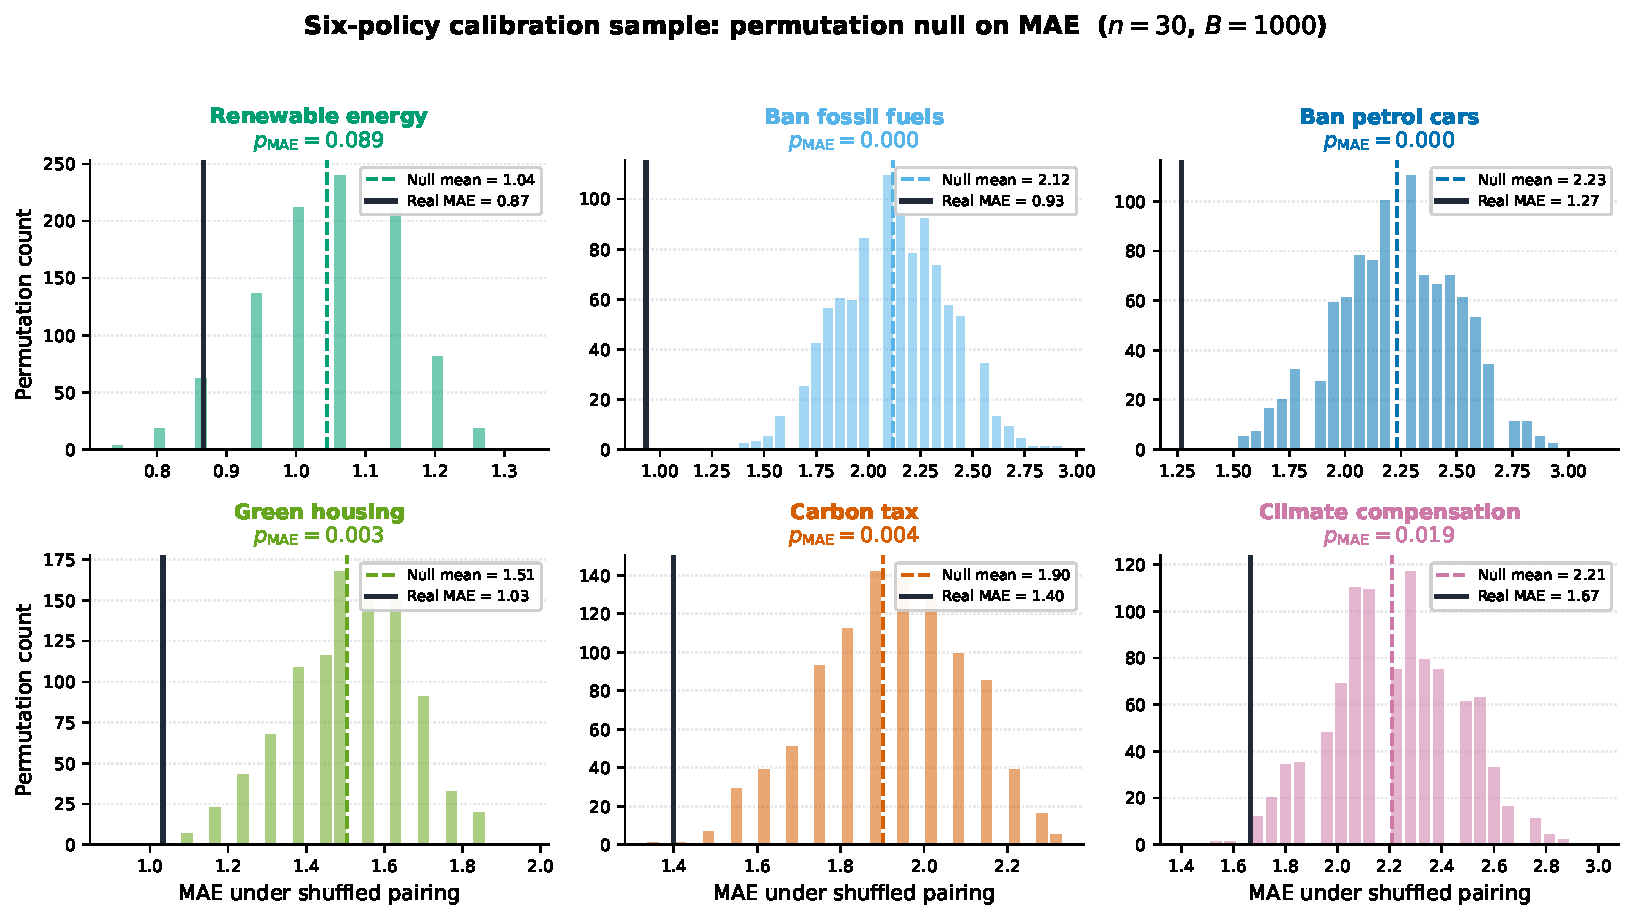
\includegraphics[width=0.98\textwidth]{figures/calib_null_sixpolicy.pdf}
  \caption{MAE-based shuffle test for persona signal by policy in the
  $n=30$ main calibration sample ($B=1{,}000$ random reassignments
  per panel; the figure was redrawn at $B=1{,}000$ for visual
  consistency, while the stored CSV in
  Table~\ref{tab:si-eval-null} uses $B=100$). The histogram shows the
  MAE that would be seen if the model's answers were randomly
  reassigned to personas; lower MAE means a closer match to the real
  respondent. The dashed line is the null mean and the solid dark
  line is the real MAE. When the dark line sits well to the left of
  the histogram, the real persona--answer pairing beats random
  pairing. That pattern appears on five of the six policies; Renewable
  energy is the only borderline case at this sample size.}
  \label{fig:si-calib-null-sixpolicy}
\end{figure*}

\begin{figure*}[t]
  \centering
  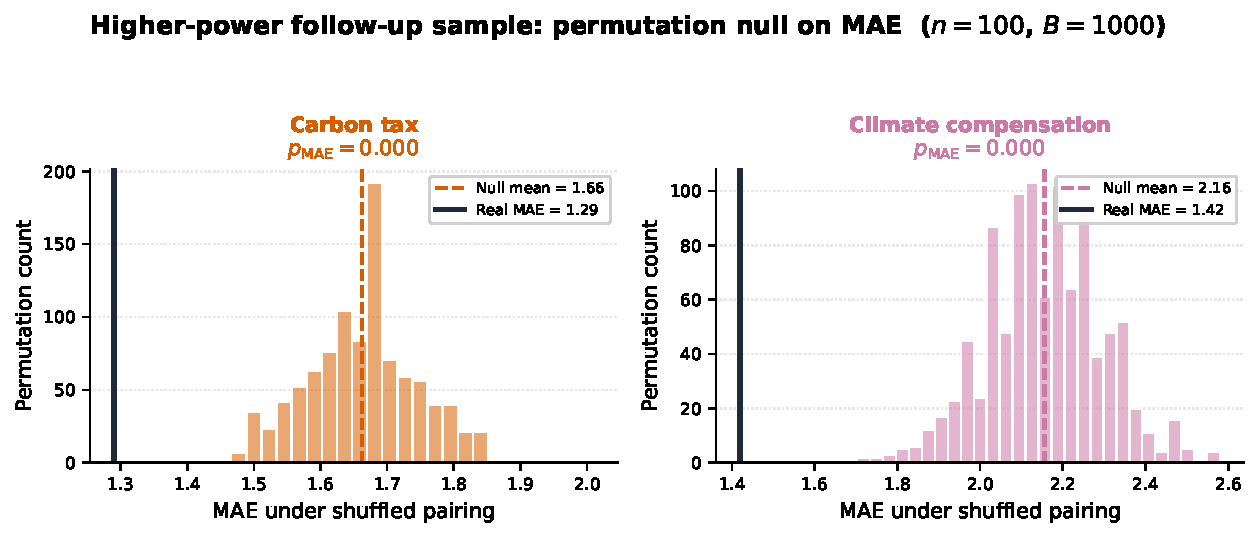
\includegraphics[width=0.85\textwidth]{figures/calib_null_followup.pdf}
  \caption{Higher-power MAE-based shuffle test for the two policies
  that were least clear in the $n=30$ sample, using a fresh $n=100$
  sample disjoint from the simulation cohort ($B=1{,}000$ random
  reassignments per panel). The same reading rule applies as in
  Fig.~\ref{fig:si-calib-null-sixpolicy}: a dark line well left of the
  histogram means the real persona--answer pairing beats random
  pairing. Both Carbon tax and Climate compensation clear that test
  comfortably, so the borderline small-sample result was a power issue
  rather than missing persona signal.}
  \label{fig:si-calib-null-followup}
\end{figure*}

\subsection{What the calibration changes in the reading of the probes}\label{subsec:si-eval-interpretation}

The calibration results do not simply say that the survey path is
``good'' or ``bad''. They separate two different properties. First, the
survey path is genuinely persona-sensitive: random reassignment usually
worsens fit, and the respondent ordering is positive on every policy.
Second, that persona sensitivity is overlaid with a policy-specific
pro-climate drift, strongest on Carbon tax and Climate compensation.

That distinction is what justifies the different evidential status of
the two probes in the main text. Probe~2 varies broadcast reach on Ban
petrol cars, the policy with the smallest stored bias in the $n=30$
calibration (+0.067), so its directional ordering is difficult to
explain as an artefact of the survey readout alone. Probe~1, by
contrast, includes Carbon tax and Climate compensation inside the
package-level index, so upward movement on those policies should be read
as the combination of simulated persuasion and a known measurement bias.
Anchoring Day~0 to the observed survey data removes that bias from the
initial condition, but it does not remove it from the Day~1 onward
readout.

\section{Useful extension paths}\label{sec:si-extensions}

The next stage of development has five main directions.

\subsection{Parallelization}\label{subsec:si-ext-parallel}

The present runs are still limited by sequential LLM calls within each
day. A practical next step is to parallelize independent calls wherever
the model logic already supports simultaneous update, especially the
generation of peer messages, broadcast reflections across recipients,
and end-of-day survey calls across agents. This would make larger
cohorts, longer horizons, and multi-seed replication more feasible
without changing the substantive design of the model.

\subsection{Stronger cognitive architecture}\label{subsec:si-ext-cognition}

The current agent design already separates persona, short-term
reflection, and tiered memory, but its cognitive architecture remains
deliberately simple. A clear extension path is to strengthen the
internal structure of the citizen agents: for example, by separating
stable values from more transient beliefs, by introducing explicit
attitude updating rules across message types, or by varying how older
reflections are compressed and recalled over longer runs.

\subsection{Persona-faithfulness improvements}\label{subsec:si-ext-persona}

The evaluation results show that the survey path is persona-sensitive
but still noisy and policy-specific in its errors. A direct next step is
to improve persona faithfulness, particularly on difficult policies such
as Carbon tax and Climate compensation. This could include prompt
refinement, alternative survey phrasing, stronger use of respondent
history in the system prompt, and further calibration tests on larger
or disjoint samples.

\subsection{Local-model and HPC options}\label{subsec:si-ext-local}

The current implementation is designed around hosted API models, but the
same framework could be extended to support local-model inference and
high-performance computing workflows. That would make it easier to run
larger experimental grids, repeated seeds, and longer horizons, and it
would provide a direct route toward more systematic model-comparison
studies under controlled compute settings.

\subsection{Next mechanism experiments}\label{subsec:si-ext-mechanisms}

The main empirical extensions are straightforward. The current design
already supports further tests of broadcast reach asymmetry, phase
ordering, peer-message intensity, and the contrast between single-policy
and package-mode persuasion. It also supports direct comparison of the
three Day~0 anchor modes and further replication across seeds, policies,
population sizes, and time horizons. These are the most immediate next
mechanism experiments for establishing which observed patterns are
stable properties of the framework rather than features of one short
run.

\backmatter

\section*{Declarations}

\begin{itemize}
\item \textbf{Funding}: % TODO
\item \textbf{Conflict of interest}: The authors declare no competing interests.
\item \textbf{Ethics approval}: Secondary analysis of an existing YouGov survey panel; no new human-subjects data collected.
\item \textbf{Data availability}: % TODO
\item \textbf{Code availability}: Source code available at \url{https://github.com/} % TODO add repo URL
\item \textbf{Author contribution}: % TODO
\end{itemize}

\bibliography{references}

\end{document}
